\chapter{Memory}


\begin{wrapfigure}{l}{1.5in}
\caption{iDecode}\label{fig:memory}
\begin{center}
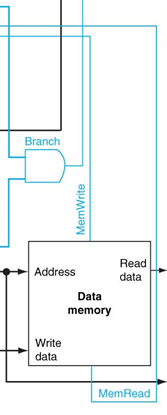
\includegraphics[width=1.5in]{../images/pipeline_memory.png}
\end{center}
\end{wrapfigure}

\WrapBarrier

\section{Branch Resolution}

We now have all the information necessary to decide if the computer should branch or not.  We have the signal `branch' to tell us if it is a branch command, and we have `zero' to tell us if the condition was met.  Both branch and zero must be true so we will combine them with an `and' gate.  And gates are a primitive in Verilog and are declared the same as a user defined module, i.e. by stating the type (and) followed by a name and then a parameter list in parenthesis.  The output is first and there can be two or more inputs.  Since it is a primitive you don't need to verify it and can just place it in the memory stage, making this a one line implementation.

\section{Data Memory}

This will be almost exactly like the instruction memory, with only two changes:
\begin{enumerate}
\item reading is now conditional on the `read' control wire being high.
\item writing is now permissible if the `write' control wire is high.
\end{enumerate}
As such, take your instruction memory (it is the right size, you could also use your register memory, but that would require more modification) and add the two changes above then test.

\section{Final Buffer}

As before the buffer is simple but tedious so I am providing it.  To save time, I am providing you a `certified' buffer, so you don't need to test it.

\section{Your Assignment}

You are to:
\begin{enumerate}
\item Instantiate the AND gate directly in the memory stage.
\item Use instruction memory as a basis for data memory, and add the two new changes.  Verify with a testbench and timing diagram.
\item Integrate data memory and the buffer into the memory stage.  Verify it works with a testbench and timing diagram.
\item  Write up a lab report in \LaTeX\ following the lab format in \verb1LabN.tex1 and generate a pdf file.
\item Upload the pdf and all the Verilog files to the course LMS.
\end{enumerate} 